% Filename: p2_advanced_vim@latex_with_vim.tex
% This code is part of LaTeX with Vim.
% 
% Description: LaTeX with Vim is free book about Vim, LaTeX and Git.
% 
% Created: 29.03.12 11:27:09 PM
% Last Change: 29.03.12 11:28:14 PM
% 
% Author: Raniere Gaia Costa da Silva, r.gaia.cs@gmail.com
% Organization:  
% 
% Copyright (c) 2010, 2011, 2012, Raniere Gaia Costa da Silva. All rights 
% reserved.
% 
% This file is license under the terms of a Creative Commons Attribution 
% 3.0 Unported License, or (at your option) any later version. More details
% at <http://creativecommons.org/licenses/by/3.0/>.
\chapter{Comandos avançados} \label{sch:vim:advance}
\section{Usando a \textit{shell}}

Para acessar a \textit{shell} sem fechar o Vim pode-se utilizar o comando \lcode{:sh}. Para retornar ao Vim deve-se utilizar os comandos \lcode{Ctrl}+\lcode{d} ou \lcode{exit}.

Para executar um comando da \textit{shell} diretamente do Vim deve-se utilizar o comando \lcode{:!} seguido pelo comando da \textit{shell}.

\section{Trabalhando com vários arquivos}
O Vim permite trabalhar com vários arquivos. Para abrir vários arquivos apresentando um em cima do outro, como apresentado na Figura \ref{fig:vim_vsplit_screen},
\begin{figure}[h!]
    \centering
    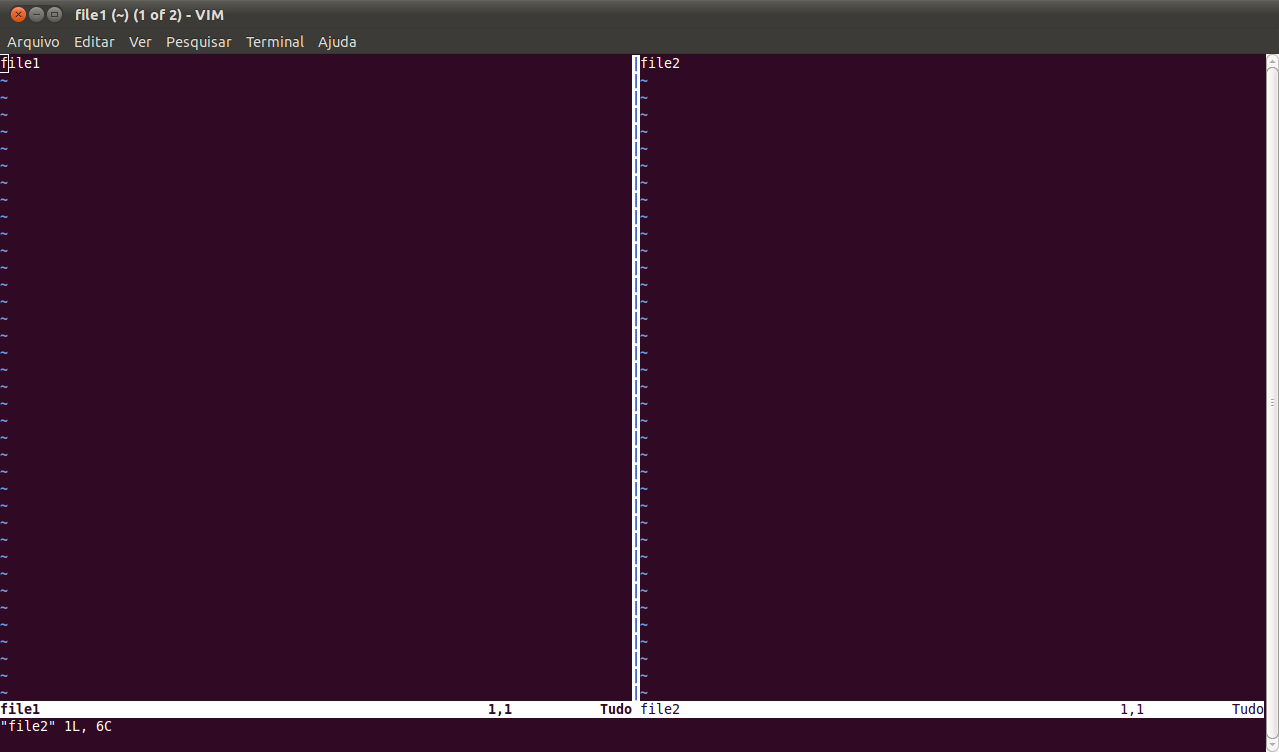
\includegraphics[height=6cm]{figures/vim_vsplit_screen}
    \caption{Dois arquivos separados verticalmente.}
    \label{fig:vim_vsplit_screen}
\end{figure}
pode-se utilizar, na \textit{shell}, o comando
\begin{code}
    vim -o file1 file2
\end{code}
e no caso do Vim já estar aberto utilizar o comando \lcode{:vsplit} .
Já para abrir vários arquivos apresentando um ao lado do outro, como apresentado na Figura \ref{fig:vim_split_screen},
\begin{figure}[h!]
    \centering
    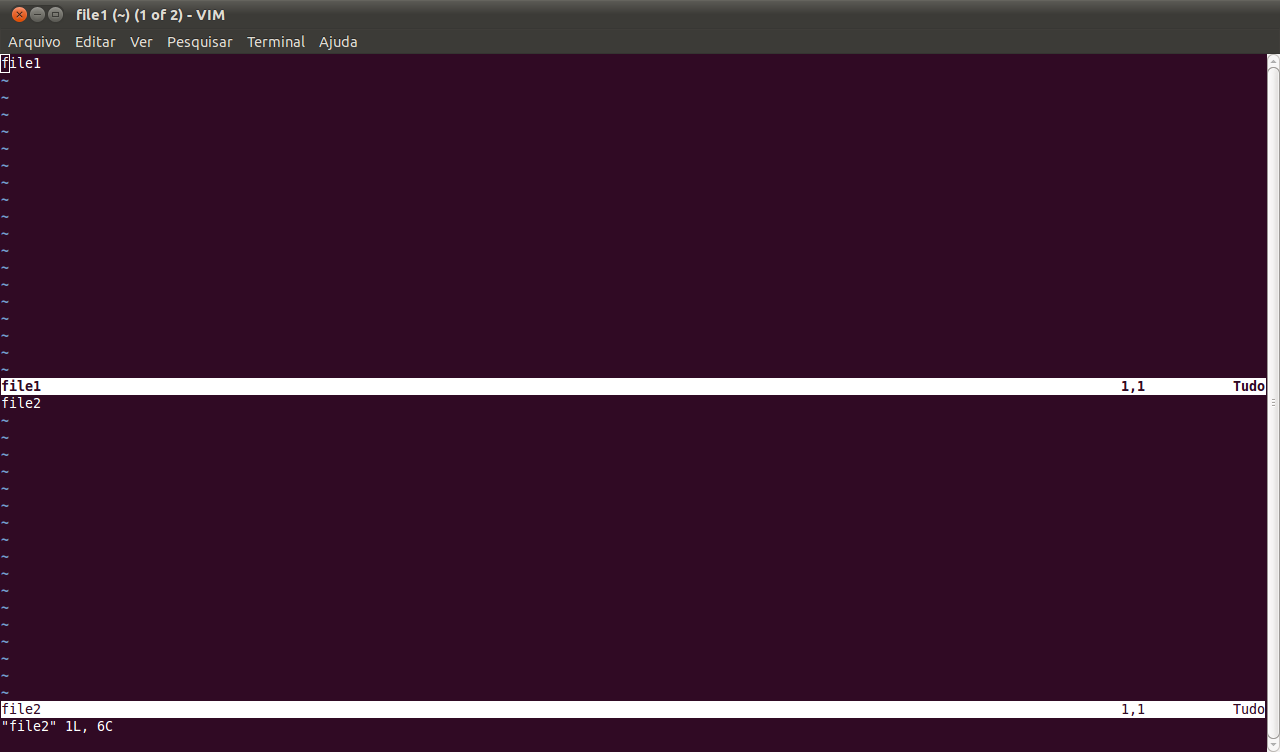
\includegraphics[height=6cm]{figures/vim_split_screen}
    \caption{Dois arquivos separados horizontalmente.}
    \label{fig:vim_split_screen}
\end{figure}
pode-se utilizar, na \textit{shell}, o comando
\begin{code}
    vim -O file1 file2
\end{code}
e no caso do Vim já estar aberto utilizar o comando \lcode{:split} .
E para apresentá-los sobrepostos pode-se utilizar, na \textit{shell}, o comando
\begin{code}
    vim file1 file2
\end{code}
e no caso do Vim já estar aberto utilizar o comando \lcode{:open} .

A movimentação entre as subjanelas ocorre pelos comandos \lcode{Ctrl}+\lcode{w} seguido da direção da ``nova'' subjanela em relação a ``antiga''. Já a movimentação os arquivos ocorre pelos comandos \lcode{:bn}, para o próximo arquivo, \lcode{:bp}, para o arquivo anterior, e \lcode{:b} seguido do número respectivo arquivo que deseja-se acessar.

Para listar os arquivos deve-se utilizar o comando \lcode{:ls}.

\section{Comparando arquivos}
Para comparar dois arquivos pode-se utilizar, na \textit{shell}, o comando
\begin{code}
    vim -d file1 file2
\end{code}
onde \lcode{file1} e \lcode{file2} são os nomes dos arquivos a serem comparados.
\begin{figure}[h!]
    \centering
    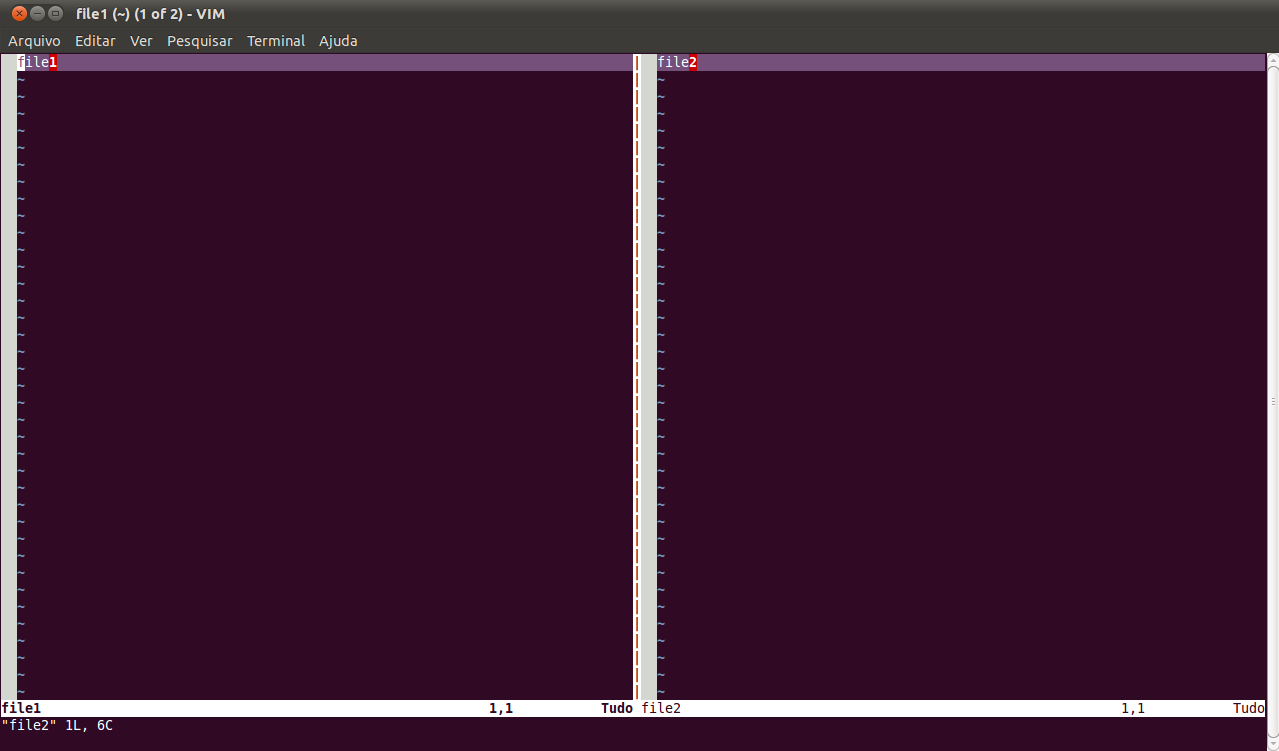
\includegraphics[height=6cm]{figures/vim_diff_screen}
    \caption{Tela de comparação de dois arquivos.}
    \label{fig:vim_diff_screen}
\end{figure}
